\documentclass[a4paper, 10pt, fleqn]{article}
\usepackage{../custom}
\usepackage{../pageformatting}
\usepackage{tikz}
\usepackage{aeguill}

\usepackage[ngerman]{babel}
%mathe packages
\usepackage{amsmath}

\graphicspath{{pdf/}{../images/}{../uml/}}

%============PAGE PROPERTIES=============
\newcommand{\revisiondate}{\today}
\newcommand{\documenttitle}{Clock Pendulum Analyzer} % used for title in title and subtitle pages
\newcommand{\authors}{Tobias Kreienbühl \& Daniel Föhn} %used for title page only
\newcommand{\subauthors}{im Auftrag der Hochschule Luzern} %used for title page only
\newcommand{\subtitle}{Sys Spec} % used for title and subtitle pages
\newcommand{\documentdesc}{System Spezifikationen des \documenttitle}
\newcommand{\dozent}{Josef Bürgler}
\newcommand{\rpi}{Raspberry Pi 3}
\newcommand{\iic}{$I^2C$}

\begin{document}
	\begin{titlepage}
		\titleGM
		\thispagestyle{empty}
	\end{titlepage}
	
	\tableofcontents
	
	\clearpage
	\section{Einführung}
		\subsection{Zweck des Dokuments}
		\subsection{Zielpublikum}
		\subsection{Versionierung}
			\begin{table}[h]
				\centering
				\begin{tabularx}{\textwidth}{|c|c|X|}
				\hline
				\rowcolor{shadecolor}\textbf{Version} & \textbf{Datum} & \textbf{Kommentar}\\ \hline
				V1.0 & \today & initial file \\ \hline
				\end{tabularx}
			\end{table}
		\subsection{Glossar}
			\begin{description}
				\item[Abkürzung]- Erklärung
			\end{description}
    
    \clearpage
    %!TEX root = SysSpec_ClockPendulumAnalyzer.tex
\section{Ausgangslage}
Eine Pendeluhr besteht grundsätzlich aus drei Komponenten: dem Energiespeicher (eine Spiralfeder
oder ein Gewicht), einer Dosiereinheit (Pendel mit Hemmung), welche die Energie portioniert an ein
Räderwerk abgibt und einer Anzeigeeinheit (das Zifferblatt).\\
\\
Die Genauigkeit einer Pendeluhr wird wesentlich bestimmt durch das Pendel. 
Durch die genaue Messung einer Periode kann der Fehler pro Tag vorausgesagt werden.
Die volle Periode eines Sekundenpendels sollte exakt 2 Sekunden betragen; dann läuft die Uhr exakt.
Eine Abweichung von 1 Millisekunde addiert sich im Laufe des Tages auf einen Fehler von ca. 43 Sekunden.\\
\\
Zur manuellen Überprüfung einer Pendeluhr wird diese meist über eine gewisse Zeitspanne, z.B. eine Woche oder ein Monat, beobachtet und dann mit einer Referenzuhr verglichen.
Dieser Vorgang ist sehr langsam und je nach Referenzzeit auch ungenau.

\section{Ziele}
Es soll ein Device erstellt werden, welches die Messung eines Pendels ermöglicht und so die Genauigkeit (Abweichung pro Tag) des Pendels direkt anzeigen kann.\\
Dabei sollen die Messungen in (Sub)-Mikrosekunden erfolgen.\\
Weiter sollen die Messdaten eines Pendels auch über längere Zeit beobachtet werden können.\\
Die Messdaten sollen visualisiert werden um die Auswertung der Daten zu erleichtern.

\section{Scope}
Dieses Projekt beschränkt sich auf das Erstellen von Funktionsmuster (Prototypen) inklusive Visualisierung der Messdaten.\\
Es werden ausschliesslich die folgenden Pendeltypen unterstützt:
\begin{itemize}
	\item Einfachpendel
	\item Doppelpendel
	\item Kreispendel (Typ Atmos)
\end{itemize}
Die Pendellänge muss zwischen 150 und 1000mm liegen, der Durchmesser bei Kreispendeln zwischen 50 und 300mm\\
Die Konstruktion eines Pendels ist nicht Teil dieses Projekts.

\section{Anforderungen}
\subsection{funktionale Anforderungen}
	\begin{itemize}
        \item Die Genauigkeit soll mit einer quadratischen Approximation erfolgen.
        \item Die Messung soll an einem Punkt vorgenommen werden.
        \item Als Referenzclock soll für Prototyp 1 eine 32kHz RTC\footnote{RTC = Real Time Clock} verwendet werden, für Prototyp 2 eine GPS- disziplinierte 10MHz RTC.
        \item Die Messvorrichtung darf keinerlei mechanische Eingriffe an dem zu messenden Pendel erfordern und soll hinter dem Pendel angebracht werden können.%unklar ob nicht-f oder funktional
        \item Die Messdaten müssen persistent gespeichert werden.
		\item Die Messdaten müssen in einem Webbrowser visualisiert werden. Es sollen die Browser Google Chrome, Firefox, Safari und Opera unterstützt werden.
		\item Die Messvorrichtung muss auf die Grösse des Pendels anpassbar sein, um verschieden grosse Pendel zu unterstützen
		\item Der Pendeltyp, der gemessen wird, soll vom Systembenutzer festgelegt werden können.
		\item Der Zeitbereich der angezeigten Daten soll vom Benutzer gewählt werden können.
		\item Die Anzeige soll sowohl auf Desktop-PC's / Notebooks, wie auch auf mobilen Geräten möglich sein.
        
		\item (Optional) Es soll die Temperatur gemessen werden, um einen allfälligen Einfluss auf die Pendelgenauigkeit anzeigen zu können.
        \item (Optional) Es soll die Luftfeuchtigkeit gemessen werden, um einen allfälligen Einfluss auf die Pendelgenauigkeit anzeigen zu können.
	\end{itemize}
\subsection{nicht-funktionale Anforderungen}
	\begin{itemize}
		\item Die Messgenauigkeit muss im Mikrosekundenbereich liegen.
        \item Die Messdaten müssen über einen Zeitraum von 3 Monaten verfügbar sein.
        \item Die Messdaten dürfen bei einem Stromunterbruch nicht verloren gehen.
		\item Die Repräsentation der Daten soll in grafischer und tabellarischer Form erfolgen.
        \item (Optional) Die Messgenauigkeit muss im Nanosekundenbereich liegen.
	\end{itemize}

\section{Resultate}
Es sind die Folgenden Resultate zu erstellen:
\begin{itemize}
	\item[\textbf{R1:}] Hardwaresystem für die Messung des Pendels.
	\item[\textbf{R2:}] Applikationssoftware auf dem Messsystem.
	\item[\textbf{R3:}] Applikationssoftware für die Darstellung der Messdaten.
	\item[\textbf{R4:}] Dokumentation.
\end{itemize}

\section{Business Case}
    Mit dem zu erstellenden Gerät kann die Abweichung einer Uhr viel effizienter gemessen werden. Der Benutzer braucht nicht mehr Stunden damit zu verbringen die Uhr zu beobachten und kann anhand der Messung die Uhr schneller nachjustieren.\\
    Weiter kann mit dem Gerät der Einfluss von Temperatur und Feuchtigkeit beachtet werden und somit eine qualitative Verbesserung der Einstellung erzeugt werden.
    
    \subtitlepage{System Spezifikation}
    %!TEX root = SysSpec_ClockPendulumAnalyzer.tex
\section{Hardware Komponenten}
Um die Pendeldurchgänge der zu messenden Uhr erfassen, vergleichen und auswerten zu können, werden diverse Hardwarebausteine benötigt. In diesem Kapitel werden die Aufgabe und Entscheidungsgrundlagen beschrieben.
\subsection{IR-Sensoren}
	Alle in Frage kommenden Sensoren für die Ermittlung der Pendeldurchgänge basieren auf optischer Technologie, da Schallsensoren nicht genau genug sind oder zu nahe am Pendel platziert werden müsten. Mechanische Sensoren können aufgrund der physikalischen Effekte auf das Pendel verworfen werden.\\
	 Bei den optischen Sensoren stellt sich die Frage, ob der Sender und der Empfänger sich im gleichen Sensor befinden und ob ein Reflektor benötigt wird oder nicht.\\
	Aufgrund der unterschiedlichen Bauarten der Pendeluhren haben wir uns bezüglich für einen Sensortyp entschieden, welcher keinen Reflektor benötigt und bei dem Sender und Empfänger sehr nahe beieinander liegen. Auf diese Weise sind auch kleine Pendel messbar und es müssen keine Reflektoren angebracht und ausgerichtet werden.\\
	Aus Kostengründen und seiner kleinen Baugrösse haben wir uns für die Reflektions-Lichtschranke SFH9201 von Osram entschieden (Abbildung \ref{fig:SFH9201}).
	\begin{figure}[H]
        \centering
        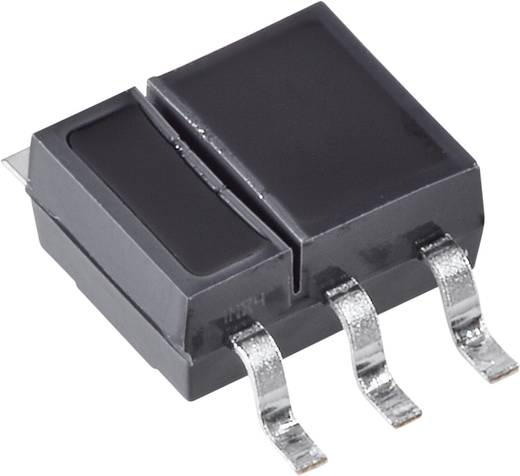
\includegraphics[width=.5\textwidth]{reflexions-lichtschranke-sfh91019201-osram-1-st}
        \caption{Reflexlions-Lichtschranke Osram SFH9201 (Bildquelle: www.conrad.ch)}
        \label{fig:SFH9201}
    \end{figure}
	Der Sender befindet sich im kleineren, oberen Rechteck und der Empfänger im Unteren. Die detaillierten Eigenschaften können dem Datenblatt im Anhang, Seite <tbd> entnommen werden. Anbei die zentralen Eigenschaften:
	\begin{table}[H]
		\begin{tabular}{|p{11cm}|p{4cm}|}\hline
			Reaktionszeit auf Auslösung (Anstiegszeit): & 50$\mu{s}$ \\ \hline
			Bauteilhöhe:								& 4.2mm\\ \hline
			Bauteilbreite:								& 6.2mm inkl Anschlusspins\\ \hline
			Optimaler Arbeitsabstand:					& 1mm bis 5mm \\ \hline
		\end{tabular}
		\caption{Übersicht der Eigenschaften der Reflektions-Lichtschranke SFH9201}
		\label{tab:SFH9201}
	\end{table}
\subsection{GPS Modul}
	Ein GPS Modul wird benötigt um den Sekundentakt exakt zu synchronisieren und so keinere Ungenauigkeiten der Messfrequenz ausgleichen zu können. Weiter dient das GPS-Modul zur Ermittlung der aktuellen Absolut-Zeit.\\
	Die Positionsfunktion des GPS-Moduls wird nicht benötigt und implementiert. Gemeinsam mit der externen Real-Time Clock ist unsere Wahl beim GPS-Modul auf ein Modell aus der Feather-Wing Familie von Adafruit gefallen (Abbildung \ref{fig:GPS3133}). Ausschlaggebend dafür sind modularität, Kosten und Funktionsumfang. Das GPS -Modul bietet direkt einen 1-Sekunden-Puls über den FIX-Pin, wenn keine GPS-Verbindung besteht sowie über den PPS-Pin bei vorhandener Verbindung. Somit ist ein Referenzsignal auch bei unterbrochener Verbindung verfügbar, wenn auch nicht mit der gleichen Genauigkeit. Die GPS-Zeitgenauigkeit ist im Datenblatt von Adafruit, Angang ab Seite <tbd> nicht angegeben, die GPS-Genauigkeit bezüglich des Sekundenpulses liegt im Bereich von <40ns (gpstime.com). Die Genauigkeit des Sekunden-Pulses im Offline-Modus ist nicht verfügbar, da nicht im Datenblatt enthalten. Für eine präzise Messung ist somit eine GPS-Verbindung Pflicht. Für funktionale Systemtests ohne Berücksichtigung der Messgenauigkeit ist der Offline-Sekundenpuls ausreichend.
		\begin{figure}[H]
        	\centering
        	\includegraphics[width=.5\textwidth]{gps_3133_top}
        	\caption{GPS-Modul Draufsicht mit den Pins PPS und FIX (Bildquelle: learn.adafruit.com)}
        	\label{fig:GPS3133}
    	\end{figure}
	Zur Nutzung des GPS Moduls zum Setzen der Systemzeit kann das GPS-Modul über UART RS232 an den RX-TX Pins ansgeschlossen und angesprochen werden.    	
\subsection{Real Time Clock}
	Die Real-Time Clock (RTC) kann als externer Frequenzgeber verwendet werden, da sie über ein 32KHz signal verfügt, welches eine Abweichung von +/- 2 ppm\footnote{Parts Per Million} auf ein \textbf{TODO: exakte Zeiteinheit für die Toleranz einfügen} verspricht.\\
	Weiter verfügt die RTC über die Möglichkeit, dem Raspberry PI die Absolutzeit zu vermitteln, wenn z.B. keine Netwerkverbindung besteht oder kein NTP\footnote{Network Time Protocol} verfügbar ist.
\subsection{Hardware Counter}
\subsection{Raspberry Pi}
Die ganze Software wird mittels C++ auf einem Raspberry Pi Version 3 (kurz RPi3) ausgeführt.

\subsubsection{Betriebssystem und Software}
Für das Betriebssystem wird ein extrem leicht gewichtetes OS verwendet. Dies verhindert dass ungewünschte daemons oder andere Programme den Betrieb verlangsamen. Es wird daher nur das allernötigste installiert. In der untenstehenden Auflistung sind alle zusätzlich installierten Programme aufgelistet. 

\begin{table}[h]
    \begin{tabular}{ll}
        ArchlinuxARM & OS für Raspberry Pi\\
        i2c-tools 3.1.2-1 & i2c tool set für Linux\\
        libconfig & C/C++ Konfiguration Datei Bibliothek\\
        libbcm2835 & Broadcom BCM 2835 c Bibliothek für Raspberry Pi\\
    \end{tabular}
    \caption{installierte Software auf dem RPi3}
\end{table}

\noindent Das Betriebssystem wird mit einem Benutzer und möglichem SSH Zugriff eingerichtet. Um per SSH auf das Raspberry zugreifen zu können muss der Host im Netzwerk 192.168.192.0/24 sein.
\begin{table}[h]
    \begin{tabular}{ll}
        Benutzer: & clockpendulum \\
        Passwort: & cpa\_admin \\
        IP: & 192.168.192.75 \\
    \end{tabular}
    \caption{Daten für den Zugriff auf das RPi3}
\end{table}
%user: clockpendulum
%pw: cpa_admin
    \clearpage
	%!TEX root = SysSpec_ClockPendulumAnalyzer.tex
\section{Systemdesign}
    Im Kapitel Systemdesign wird die Umsetzung einzelner Komponenten sowie der gesamte Kontext des CPA erklärt.
        \subsection{Kontextdiagramm}
        Der CPA Kontext wird mittels untenstehendem Diagramm dargestellt. Das Projekt umfasst ein tinyK20 als Hardware Counter, ein Raspberry Pi als Recheneinheit und ein Sensor Board auf dem ein Infrarotsensor montiert ist.\\
        Für die Benutzerinteraktion wird ein UserInterface definiert und ein Web Client erstellt. Das UserInterface ermöglicht es weitere Benutzerschnittstellen an den CPA zu hängen. Zum Beispiel eine Qt Applikation.
        \begin{figure}[H]
            \centering
            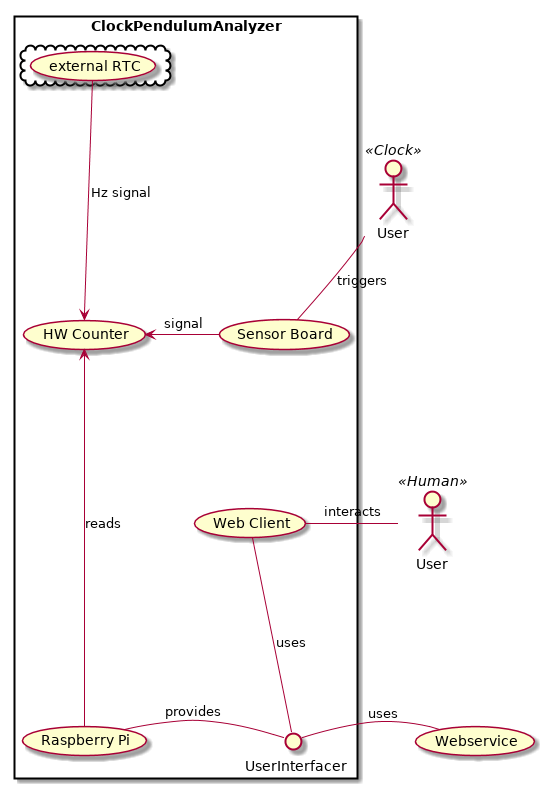
\includegraphics[width=.7\textwidth]{context.png}
            \caption{erweitertes Kontextdiagramm}
            \label{fig:kontext}
        \end{figure}

    	\subsection{Umsetzung des Clock Update} %TODO deprecated?
        \clearpage
        % !TEX root=SysSpec_ClockPendulumAnalyzer
\subsection{Umsetzung des GPIO Zugriff}
Der Zugriff auf die GPIO Pins des \rpi\ wurde mit einer simplen Klasse umgesetzt. Diese Klasse ist verantwortlich für das Exportieren und Unexportieren der Pins.
Dies geschieht bei der Initialisierung der Klasse beziehungsweise beim Dekonstruktor. Dabei wird das Prinzip der ''Resourcenbelegung ist Initialisierung'' (kurz RAII) nicht verletzt.\\
\\
Die Aufgaben des Benutzers sind nur Richtung setzen und dann Lesen bzw. Schreiben der Pins. Die Richtung (Output / Input) kann zur Laufzeit geändert werden.

\subsubsection{Pinbelegung}
Die Pinbelegung auf dem \rpi\ wird in Bild \ref{fig:pi_belegung} gezeigt.
\begin{figure}[H]
    \centering
    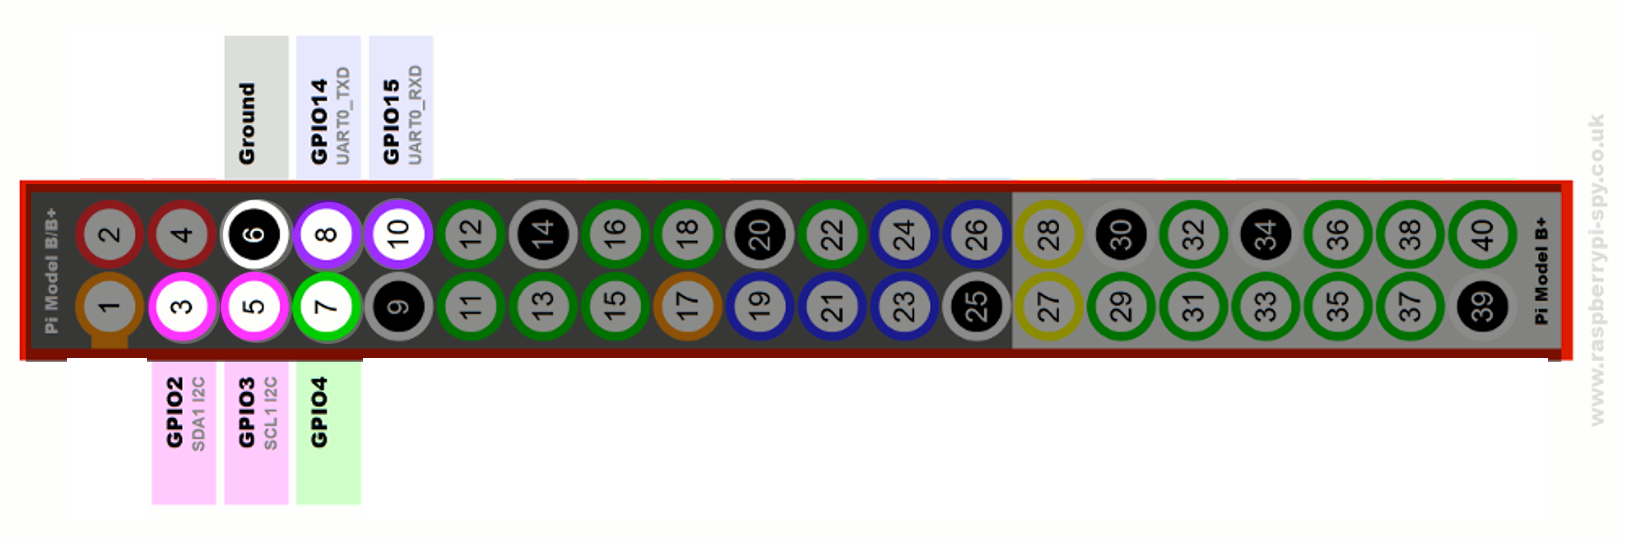
\includegraphics[width=\textwidth]{pinbelegung}
    \caption{Pinbelegung des \rpi\ (Originalbild von www.raspberrypi-spy.co.uk)}
    \label{fig:pi_belegung}
\end{figure}

\noindent Pin 6,8,10,3 und 5 werden nicht durch die GPIO\footnote{General Purpose Input Output} Klasse angesteuert. Diese sind für die UART beziehungsweise \iic\ Kommunikation reserviert, die in den nachfolgenden Kapitel \ref{sec:i2c} und \ref{sec:uart} beschrieben sind.\\\\
Pin 7 dient als Interrupt-Pin für den Zähler. Dieser wird bei Programmstart als High Output Pin gesetzt um damit den Zähler zurückzusetzen. Damit wird erreicht, dass das System auf unterschiedliche Aufstartzeiten reagieren kann und die ganze Messung gleichzeitig starten kann. Der Zähler-Reset wird nur bei Programmstart ausgeführt und danach nicht mehr.

\subsubsection{\iic\ Implementierung}\label{sec:i2c}
Der \iic\ Anschluss läuft über Pin 3 (SDA\footnote{Data Signal}) und 5 (SCL\footnote{Clock Signal}).\\
Für den \iic\ wurde ebenfalls eine abstrahierende Klasse entwickelt. Diese verwendet die bereits vom Linux bereitgestellten Funktionalitäten zum Lesen und Schreiben von \iic-Geräten.\\
\\
Im Kontext des \documenttitle\ ist der \iic\ Bus als Kommunikation zwischen RTC, Zähler und \rpi\ gedacht. 
Dabei wäre das \rpi\ der Master und fordert die anderen zwei Teilnehmer nach ihren Daten.

\paragraph{Aufgetretene Probleme:}
Aufgrund des gewählten Betriebssystem und der dadurch entstandenen Problematik mit der Schnittstelle auf dem \rpi, wird die \iic\ Implementierung nicht beendet.\\
Die Problematik bestand darin, dass die \iic-Geräte auf dem Linux nicht erkannt wurden. Nach mehreren Versuchen die Geräte zu erkennen, wurde entschieden, dass zur Kommunikation eine USB-UART Verbindung aufgebaut wird. Diese Verbindung beinhaltet nur noch die Kommunikation mit dem Zähler des \hwb s. Mehr zum UART ist im folgenden Kapitel \ref{sec:uart} zu lesen.

\clearpage
\subsubsection{UART Implementierung}\label{sec:uart}
Für das Lesen des GPS Signals wird eine UART Kommunikation benötigt.
Aufgrund der \iic\ Problematik wird die GPS UART Verbindung auf den zwei Pins 8 und 10 nicht weiter verfolgt.\\
\\
Dafür wird eine USB-UART Verbindung zum \hwb\ realisiert. Als Übertragungsmedium dient ein micro-USB Kabel und lässt daher nur eine 1-zu-1 Verbindung zu.\\
\\
Der Code basiert auf einer bereits implementierten Lösung aus einem früheren Projekt und wird auf die Bedürfnisses dieser Kommunikation angepasst.\\
Das Lesen des UARTs findet in einem eigenen Thread auf dem \rpi\ statt und empfängt Signale, die vom \hwb\ gesendet werden. Wenn eine Nachricht empfangen wird, wird diese an einer Liste angehängt. Nebenbei läuft der Main-Thread und liest, wenn die Liste einen Eintrag enthält, den Zeitstempel und dessen absolute Zeit aus. Danach wird dieser Eintrag aus der Liste entfernt.
		\subsection{Umsetzung des Hardware Counter} %TODO Hardware Counter Prinzip erklären
        \clearpage
        %!TEX root = SysSpec_ClockPendulumAnalyzer.tex
\subsection{Umsetzung der Datenpersistenz}
    Hier stehen Details zur Umsetzung der Datenspeicherung auf dem Raspberry Pi.
    \subsubsection{Datenspeicher}
    Da das Operationssystem des Raspberry Pi auf einer SD Karte gespeichert ist, empfiehlt es sich eine Alternative zu finden. SD Karten sind nicht für häufige Schreibzyklen ausgelegt. Für den Clock Pendulum Analyzer wird deshalb ein USB Speicher verwendet. Auf diesem wird die ganze Datenbank abgelegt.\\
    Der Datenspeicher wird beim Autostart über die \textit{/etc/fstab} Datei automatisch eingebunden.
    
    \subsubsection{SQLite als Datenbank}
    C++ bietet eine grosszügige Schnittstelle für SQLite Datenbanken. Durch SQLite braucht die Applikation auch keine umständliche Datenbankinstallation wie es bei MySQL der Fall wäre, da SQLite nur normale Dateien zum Aufbau verwendet.
    
    \subsubsection{Architektur und Beispielverwendung}
    Die Software speichert die folgenden Daten in einer einzelnen Tabelle ab.
    \paragraph{clock:}
    Der Wert in \textit{clock} hält den Namen fest der Uhr, von der die weiteren Daten stammen. Dieser wird beim Programmstart mitgeteilt.\\
    Das Feld ist vom Typ TEXT und besteht aus alphanumerischen Zeichen die der Regular Expression $$[a-zA-Z0-9]\{1,\}$$
    \paragraph{date:}\label{sec:db_date}%TODO datumsformat anpassen +zeit
    In diesem Feld steht der Zeitpunkt zu welchem der Datenwert entnommen wurde. Dazu wird die Systemzeit des RPi3 gespeichert und anschliessend so konvertiert, dass der Zeitstempel im Format \textbf{yyyyMMdd} gespeichert werden kann\\
    Das Feld ist vom Typ INTEGER und entspricht der Regular Expression
    $$[0-9]\{8\}$$
    \paragraph{absolutetime:}
    Hier steht der aktuell gemessene Zeitwert in absoluter Zeit. Der Wert bezieht sich auf die aktuell vergangenen Nanosekunden in einem Tag. Er startet bei 0:00 und läuft einen Tag.\\
    Das Feld ist vom Typ INTEGER und entspricht der Regular Expression
    $$[0-9]\{1,15\}$$
    \paragraph{heat:}
    Das Feld heat wird für den optionalen Teil Temperatureinfluss benötigt. Zum jetzigen Zeitpunkt ist dieses Feld mit 0 initialisiert.
    Das Feld ist vom Typ INTEGER und entspricht der Regular Expression
    $$[0-9]\{1,2\}$$
    \paragraph{humidity:}
    Das Feld humidity wird für den optionalen Teil Feuchtigkeitseinfluss benötigt. Zum jetzigen Zeitpunkt ist dieses Feld mit 0 initialisiert.
    Das Feld ist vom Typ INTEGER und entspricht der Regular Expression
    $$[0-9]\{1,2\}$$
    %TODO beispielverwendung einfügen
        \clearpage
        \subsection{Umsetzung des UI} %TODO UI Implementierung update nach Entwicklung
Die grafische Darstellung der ermittelten Messdaten wird in den folgenden Kapitel beschrieben.

\subsubsection{Webbrowser Client} 
Nach Aufgabenstellung wird ein web basierender Zugriff auf die ermittelten Messdaten gefordert. Dieser ist im Kontextdiagramm (Bild \ref{fig:kontext}) innerhalb der Systemgrenze als Web Client definiert.\\
Unter einem Web Client ist eine, auf dem Browser laufende Applikation zu verstehen.\\
\\
Der Zugriff auf die Messdaten läuft über die wohl definierte REST Schnittstelle, welche im Kapitel \ref{sec:rest} genauer erklärt ist. Dieser gekapselte Zugriff ermöglicht es eine unabhängige Darstellung zu implementieren.\\
Weiter gibt es die Möglichkeit andere grafische Benutzeroberflächen zu entwickeln, welche die gleichen Datengrundlagen haben.\\
\\
Der Aufbau des Clients erfolgt mittels eines Bootstrap Templates\footnote{Bootstrap Template von \cite{bootstrap}}. Im oberen Bereich wird die Temperatur, Feuchtigkeit, aktuelle Abweichung und Abweichung seit Beginn dargestellt. Darunter folgt ein Liniendiagramm, das den Ablauf der Abweichung pro Tag darstellt.Daneben ist eine Tagestabelle, die die Messergebnisse eines Tages anzeigt.\\
Das Liniendiagramm sowie die Tagestabelle können nach Datum gefiltert werden.

\begin{figure}[H]
    \centering
    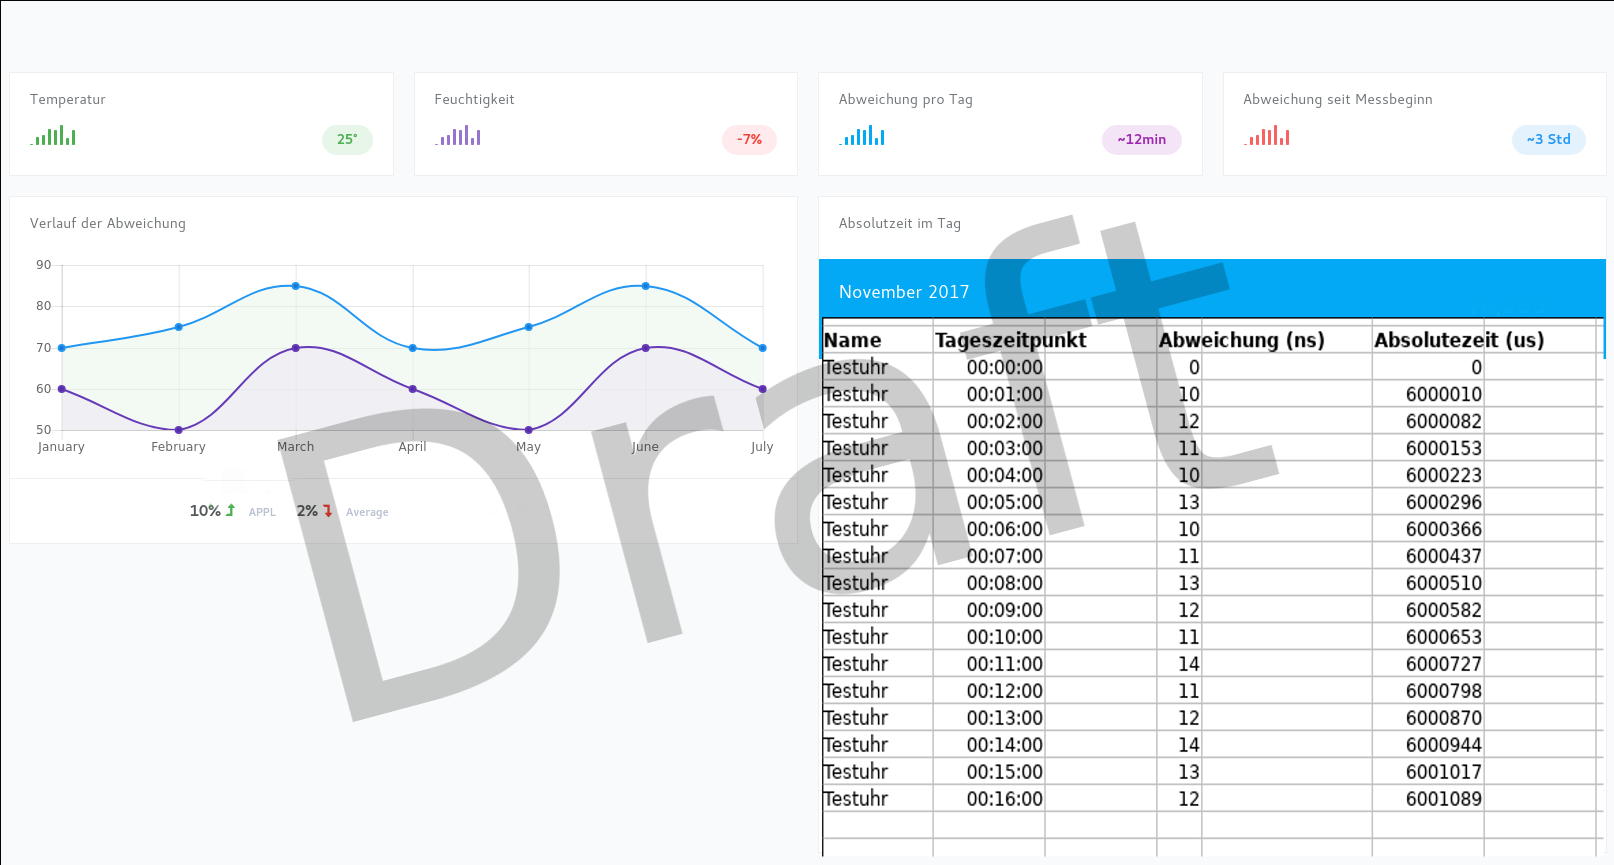
\includegraphics[width=\textwidth]{webclient_draft}
\end{figure}
        \clearpage
        %!TEX root = SysSpec_ClockPendulumAnalyzer.tex
\subsection{Sequenzdiagramm}
In diesem Kapitel werden einzelne Arbeitsabläufe anhand eines Sequenzdiagrammes dargestellt.
	\subsubsection{Start und Speichern einer Datenmessung}
    Dieses Sequenzdiagramm (Abbildung \ref{fig:sequence_save}) zeigt den Ablauf der Hauptfunktionalität.
    Zuerst werden alle zusätzlich benötigten Teilnehmer gestartet.
    Danach beginnt der Speichervorgang einzelner Datenmessungen.
    Dabei ruft das Programm die FIFO\footnote{First In, First Out}-Liste ab, welche durch die UART Kommunikation mit Messwerten befüllt wird.
    Sind 5 Datentupel aus der FIFO Liste gelesen, werden diese in der Datenbank gespeichert.
    \begin{figure}[H]
        \centering
        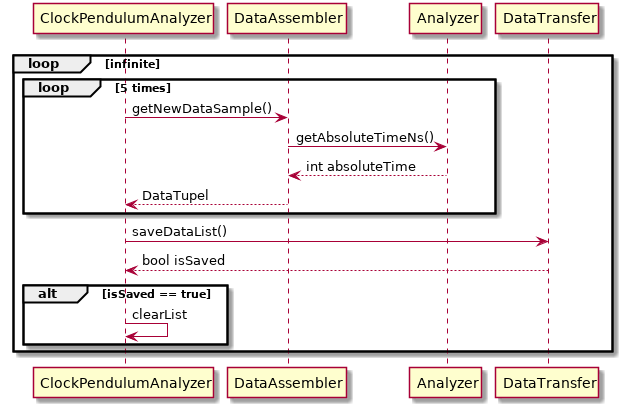
\includegraphics[width=\textwidth]{sequence_data_save.png}
        \caption{Sequenzdiagramm zum Speichern der Daten}
        \label{fig:sequence_save}
    \end{figure}

    \clearpage
    \subsubsection{Abrufen einer Datenmessung}
    Ein Webclient ruft Daten über eine HTTP Request auf die angebotene REST Schnittstelle.
    Als Antwort erhält er eine JSON Struktur der Messdaten.
    Das ganze wird im Sequenzdiagramm (Abbildiung \ref{fig:sequence_get}) unten abgebildet (mit dem Uhrennamen-Parameter als Beispiel).
    \begin{figure}[H]
        \centering
        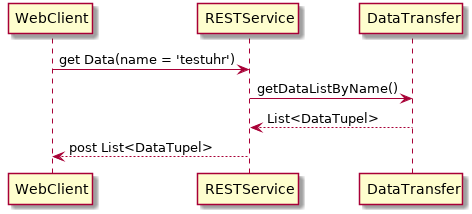
\includegraphics[width=.7\textwidth]{sequence_data_access.png}
        \caption{Sequenzdiagramm zum Aufrufen der Daten}
        \label{fig:sequence_get}
    \end{figure}
    %
	\subsubsection{Zählersystem}
	Die Software auf dem \hwb ist in C geschrieben und somit nicht objektorientiert. Dementsprechend sind die einzelnen Lebenslinien keine Objekte sondern eigene C-Dateien, deren Methoden entsprechend dem Diagramm aufgerufen werden. Die Akteure stellen dabei die Interrupt-Eingänge dar.
	\begin{figure}[H]
   		\centering
        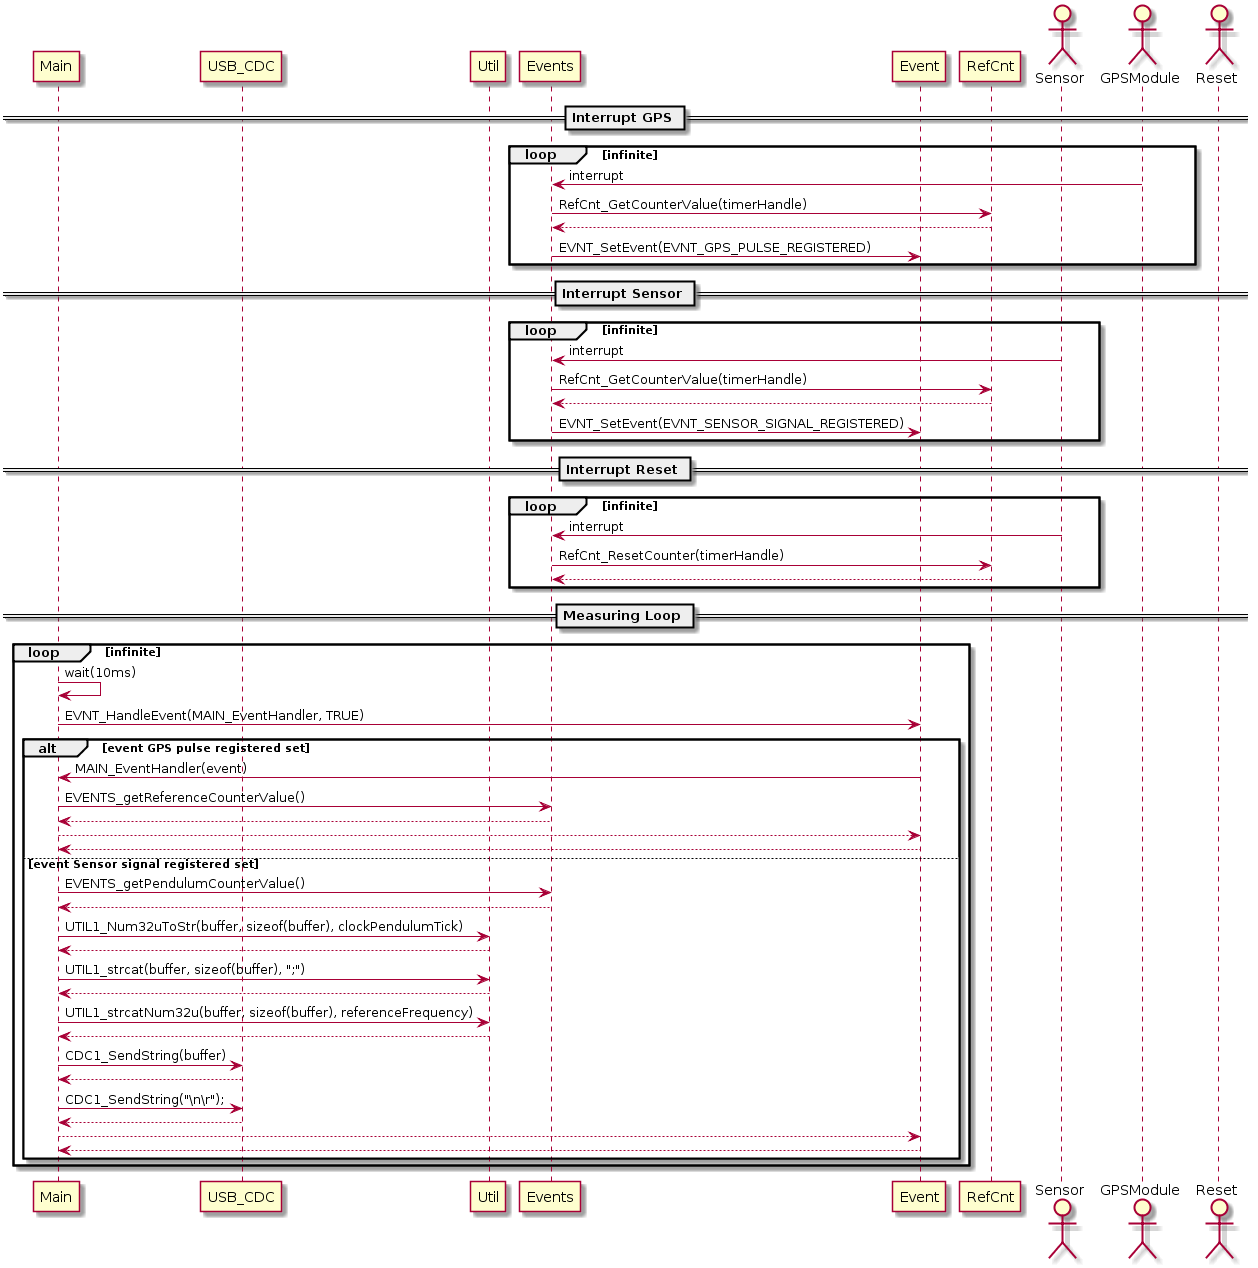
\includegraphics[width=.7\textwidth]{sequence_hwb.png}
        \caption{Sequenzdiagramm Zählersystem zur Pendelerfassung}
        \label{fig:sequence_hwb}
    \end{figure}
	\noindent Der Main-Loop, das eigentliche C-Programm, prüft alle 10 Millisekunden, ob ein Event gesetzt ist, oder ob noch Daten im USB-Kanal zum Senden vorhanden sind. Dementsprechend ist dieser Teil des Programmes nicht besonders zeitkritisch und kann problemlos zwischen den Interrupts durch das GPS-Modul und den Sensor verarbeitet werden.\\
	Die Interrupts des GPS-Moduls sind zeitkritisch und wie im Abschnitt \ref{cap:counter_realisation} beschrieben, von der höchsten Priorität. Da werden auch die aktuellen Zählerwerte umgehend gespeichert und anschliessend der entsprechende Event gesetzt, welcher dann beim nächsten Durchgang des Main-Loops verarbeitet wird. Der gesamte Ablauf ist im Sequenzdiagramm in Abbildung \ref{fig:sequence_hwb} dargestellt.

   	
        \clearpage
		%!TEX root = SysSpec_ClockPendulumAnalyzer.tex
\subsection{Klassendiagramm}
Die Klassen der Software arbeiten nach dem folgenden Klassendiagramm. Es umfasst eine Implementierung der REST Definition und Klassen für die Datenbankanbindung an SQLite.
\begin{figure}[H]
    \centering
    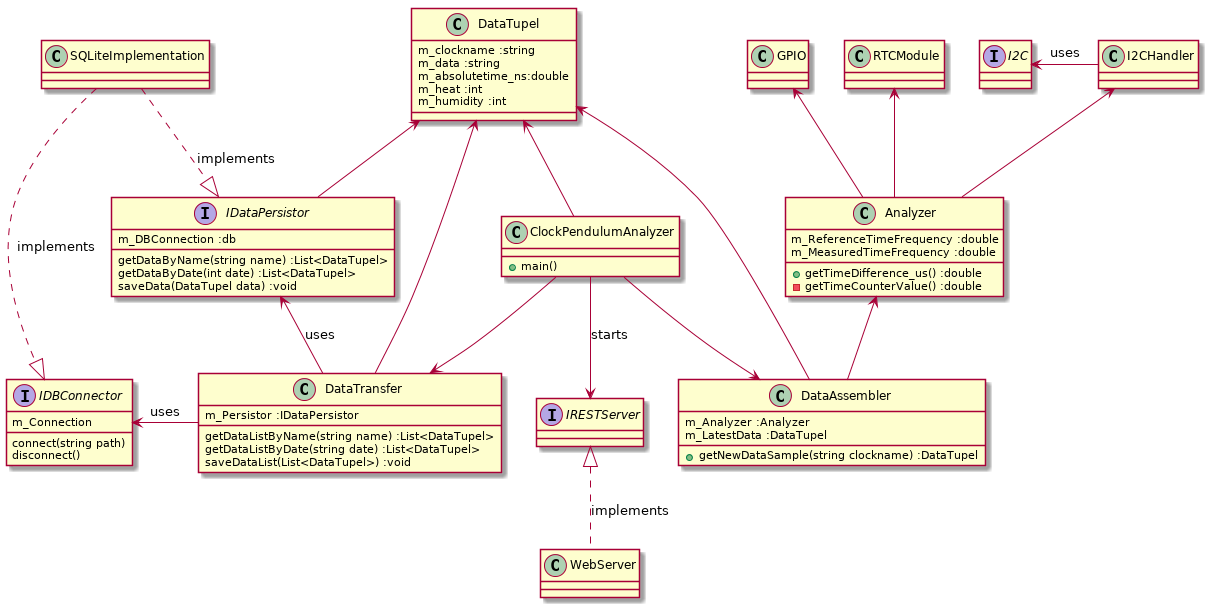
\includegraphics[width=\textwidth]{classdiagramm.png}
    \caption{Klassendiagramm der C++ Software auf dem Raspberry Pi}
\end{figure}
\subsubsection{Klassdetails}
    %TODO subject to change
	\begin{description}
        \item[ClockPendulumAnalyzer] Dies ist die Main Klasse. Sie startet alle Aufgaben.
        \item[I2CHandler] Diese Klasse öffnet und schliesst den $I^2C$-Bus und liest Daten von daran angeschlossenen Geräten.
        \item[GPIO] Eine Klasse die für das Arbeiten mit GPIO Pins auf dem Raspberry Pi zuständig ist.
        \item[Analyzer] Die Klasse ist für die Berechnung der Zeitdifferenz in Nanosekunden zuständig. Es kann auch die Differenz in Mikro- und Millisekunden ausgegeben werden.
        \item[DataAssembler] Die Klasse ist für das Zusammenfügen von Name (aus der Main Klasse) und den einzelnen Dateninputs aus dem Analyzer zuständig. Im Sequenzdiagramm ist dieser Ablauf dargestellt. 
        \item[DataTransfer] Diese Klasse ist für den Transport der DataTupel zwischen Webserver, Mainklasse und Datenbank zuständig.
        \item[DataTupel] Ein Daten Transfer Objekt (DTO) als Abstraktion der gemessenen Daten zu einem gegebenen Zeitpunkt. Beinhaltet Datum+Zeit, Name, Differenz und Werte für Feuchtigkeit und Wärme.
        \item[SQLiteImplementation] Die Implementierung der Schnittstelle \textit{IDataPersistor} und der \textit{IDBConnector} auf eine SQLite Umgebung.
    \end{description}

    \clearpage
    %!TEX root = SysSpec_ClockPendulumAnalyzer.tex
\section{Schnittstellen}
\subsection{REST Interface}\label{sec:rest}
    
    \clearpage
    %BIBLIOGRAPHY
    \nocite{*}
    \bibliography{../bibliography}
    \bibliographystyle{apacite}
    
    
    \listoffigures
    \listoftables
\clearpage
\thispagestyle{empty}
	\section*{Anhang}
\end{document}
